\documentclass[conference]{IEEEtran}
\IEEEoverridecommandlockouts
% The preceding line is only needed to issue \thanks blocks if have them.
\usepackage{cite}
\usepackage{amsmath,amssymb,amsfonts}
\usepackage{algorithmic}
\usepackage{graphicx}
\usepackage{textcomp}
\usepackage{xcolor}
\usepackage{booktabs}
\usepackage{multirow}
\usepackage{array}
\usepackage{hyperref}
\usepackage{pgfplots}
\pgfplotsset{compat=1.18}

\def\BibTeX{{\rm B\kern-.05em{\sc i\kern-.025em b}\kern-.08em
    T\kern-.1667em\lower.7Eex\hbox{E}\kern-.125emX}}

\begin{document}

\title{GazeSpeak: A Low-Cost, Step-Based Eye-Gaze Communication and Interactive AAC Framework Powered by MediaPipe Iris Tracking and Hybrid LLM Inference}

\author{
\IEEEauthorblockN{Dr. G Manjula}
\IEEEauthorblockA{\textit{Dept. of Computer Science and Design} \\
\textit{Dayananda Sagar Academy of Technology and Management}\\
Bengaluru, Karnataka, India \\
gmanjula@dsatm.edu.in}
\and
\IEEEauthorblockN{Chaitra B V}
\IEEEauthorblockA{\textit{Dept. of Computer Science and Design} \\
\textit{Dayananda Sagar Academy of Technology and Management}\\
Bengaluru, Karnataka, India \\
cbelavadi21@gmail.com}
\and
\IEEEauthorblockN{Prajwal J D}
\IEEEauthorblockA{\textit{Dept. of Computer Science and Design} \\
\textit{Dayananda Sagar Academy of Technology and Management}\\
Bengaluru, Karnataka, India \\
prajwaljd.work@gmail.com}
\vspace{0.8em}
\and
\IEEEauthorblockN{Bindu Madhuri}
\IEEEauthorblockA{\textit{Dept. of Computer Science and Design} \\
\textit{Dayananda Sagar Academy of Technology and Management}\\
Bengaluru, Karnataka, India \\
bindumadhuri.work@gmail.com}
\and
\IEEEauthorblockN{Tanvi Kulkarni}
\IEEEauthorblockA{\textit{Dept. of Computer Science and Design} \\
\textit{Dayananda Sagar Academy of Technology and Management}\\
Bengaluru, Karnataka, India \\
tanvikulkarni.work@gmail.com}
}

\maketitle

\begin{abstract}
ALS, Locked-in Syndrome, and brainstem stroke leave eye movement as the only remaining motor
channel for many patients. Commercial eye-gaze AAC systems cost \$5,000--\$15,000 and require
infrared hardware. Cheaper webcam-based alternatives suffer from the ``Midas Touch'' problem:
because gaze naturally scans the screen, continuous 2D cursor mapping fires accidental key presses
constantly. This paper presents GazeSpeak, a software-only AAC system that runs on a standard RGB
webcam. Instead of a continuous cursor, gaze is mapped to three discrete horizontal zones.
Looking left or right steps the keyboard highlight by one key; looking straight ahead arms a
dwell timer that selects the highlighted key after 800\,ms. A three-point calibration, completed
in under ten seconds, sets personalized zone thresholds using IQR outlier filtering. A hysteresis
filter ($N=2$ frames) stops brief eye flinches from triggering steps. For text entry, GazeSpeak
uses a local frequency dictionary for instant completions and Groq Llama-3.3 70B for
context-aware word prediction and abbreviation expansion (e.g., ``ftk'' to ``from the kitchen'').
A binary conversation mode lets a caregiver ask a question; the LLM generates two short answer
cards and the patient selects by gaze direction, narrowing intent over two to three rounds. Rapid
blinks ($\ge 5$ in 4\,s) trigger an audible siren and a Twilio SMS to the caregiver. The vision
pipeline runs at 18.4\,ms per frame. Emergency blink detection reaches an F1 of 0.904. Typing
throughput rises from 2.8 WPM (raw gaze) to 11.4 WPM with LLM abbreviation expansion and
22.5 WPM in binary conversation mode, with a Keystroke Savings rate of 84.2\%.
\end{abstract}

\begin{IEEEkeywords}
Assistive Communication, ALS, Eye-Gaze Tracking, MediaPipe Iris Detection, Large Language Models (LLM), AAC, Abbreviation Expansion, Emergency SOS.
\end{IEEEkeywords}

\section{Introduction}
ALS, brainstem stroke, and high-level spinal cord injuries destroy voluntary muscle control while
leaving cognition intact \cite{murray2021global}. In late-stage ALS, eye movement is often the
only remaining motor channel, which is why eye-gaze AAC systems exist \cite{lugaresi2019mediapipe}.

Four problems limit how widely these systems are used in practice.
First, commercial gaze trackers (Tobii Dynavox, Smartbox Grid) cost \$5,000--\$15,000 because
they need active infrared illuminators and high-speed cameras \cite{abilkaiyrkyzy2024dialogue}.
Second, cheaper webcam-based systems map raw gaze to a screen cursor. Because gaze naturally
scans the screen to read the UI, the cursor fires accidental key presses continuously, a problem
called the Midas Touch \cite{soukupova2016real}.
Third, standard calibration requires the patient to fixate on 9--16 grid targets in sequence,
which is exhausting for people with nystagmus or low eye movement range \cite{trnka2009user}.
Fourth, letter-by-letter typing averages fewer than 3 WPM without language prediction, which
makes long sentences impractical \cite{singh2025innovative}.

GazeSpeak addresses all four problems. It runs on a standard RGB webcam, uses a three-point
calibration that takes under ten seconds, and replaces the cursor with a step-based navigation
model that eliminates accidental selections. An LLM layer raises effective throughput to
22.5 WPM. This paper's main contributions are:

\begin{enumerate}
    \item A discrete step-based gaze navigation model where left/right gaze steps the keyboard
          highlight by one key and center gaze arms the dwell timer, removing the Midas Touch
          problem by design.
    \item A three-point horizontal calibration with IQR outlier filtering that adapts zone
          thresholds to each patient's eye movement range in under ten seconds.
    \item A two-tier language engine combining an instant local dictionary with asynchronous
          Groq Llama-3.3 70B for word prediction, abbreviation expansion, and a binary
          conversation mode.
    \item A rapid-blink emergency alert that counts blinks in a sliding 4-second window and
          triggers an audible siren plus a Twilio SMS when five or more blinks are detected.
\end{enumerate}

% ==========================================
% SECTION II: BACKGROUND & RELATED WORK
% ==========================================
\section{Background and Related Work}

\subsection{Eye Tracking in Assistive Communication}
Infrared eye trackers measure the vector between the pupil center and corneal glints from an
active IR illuminator \cite{abilkaiyrkyzy2024dialogue}. They reach sub-degree accuracy but cost
tens of thousands of dollars. Webcam-based alternatives use facial landmark libraries such as
Dlib or MediaPipe. Their gaze estimates carry spatial jitter of $2^\circ$--$4^\circ$, which is
too noisy for continuous 2D cursor control on small keyboard keys \cite{lugaresi2019mediapipe}.
GazeSpeak sidesteps this by treating gaze as a three-zone discrete signal rather than a
continuous coordinate.

\subsection{Predictive AAC and Language Modeling}
AAC typing speed research has moved from n-gram models (Dasher, GazeTalk) to LLM-based
completion \cite{trnka2009user}. LLMs generate contextually relevant predictions from prior
dialogue \cite{chen2025detecting, singh2025innovative}. GazeSpeak uses a two-tier approach:
the local dictionary returns results in under 1\,ms, and a background thread calls
Groq Llama-3.3 70B when a network connection is available, replacing local predictions
without blocking the UI.

\subsection{Blink Detection and Safety}
Soukupov{\'a} and {\v{C}}ech \cite{soukupova2016real} defined the Eye Aspect Ratio (EAR) as
the ratio of vertical to horizontal eye landmark distances. EAR drops below a threshold during
a blink and recovers when the eye reopens. GazeSpeak uses the same measure to separate
physiological blinks from deliberate rapid-blink SOS signals.

\begin{table}[htbp]
\caption{Comparative Analysis of AAC Eye-Tracking Frameworks}
\label{tab:comparative_aac}
\centering
\begin{tabular}{lcccc}
\toprule
\textbf{Feature / Metric} & \textbf{Tobii Dynavox} & \textbf{Webcam 2D} & \textbf{GazeSpeak (Ours)} \\
\midrule
Hardware Cost & \$5,000--\$15,000 & \$10--\$30 & \textbf{\$10--\$30 (RGB Webcam)} \\
Calibration Points & 9--16 Points & 9--16 Points & \textbf{3 Horizontal Points} \\
Navigation Mode & Continuous 2D & Continuous 2D & \textbf{Discrete Step-Based} \\
Midas Touch Risk & Moderate & Extremely High & \textbf{Near Zero (Center Arming)} \\
Abbreviation Expansion & No & Rule-based & \textbf{Context-Aware LLM} \\
Binary Conversation Mode & No & No & \textbf{Yes (Llama-3.3 70B)} \\
Emergency SOS Siren/SMS & External Button & None & \textbf{Automated EAR Blink SOS} \\
\bottomrule
\end{tabular}
\end{table}

% ==========================================
% SECTION III: SYSTEM DESIGN AND METHODOLOGY
% ==========================================
\section{System Design and Methodology}

\subsection{System Architecture}
The software architecture of GazeSpeak follows a multi-threaded, signal-driven modular design
developed in Python 3.13 and PyQt6. Fig.~\ref{fig:dataflow} shows the data flow between modules.
Fig.~\ref{fig:sysarch} shows the full modular system architecture across three layers: inputs,
processing, and external services.

\begin{figure}[htbp]
\centering
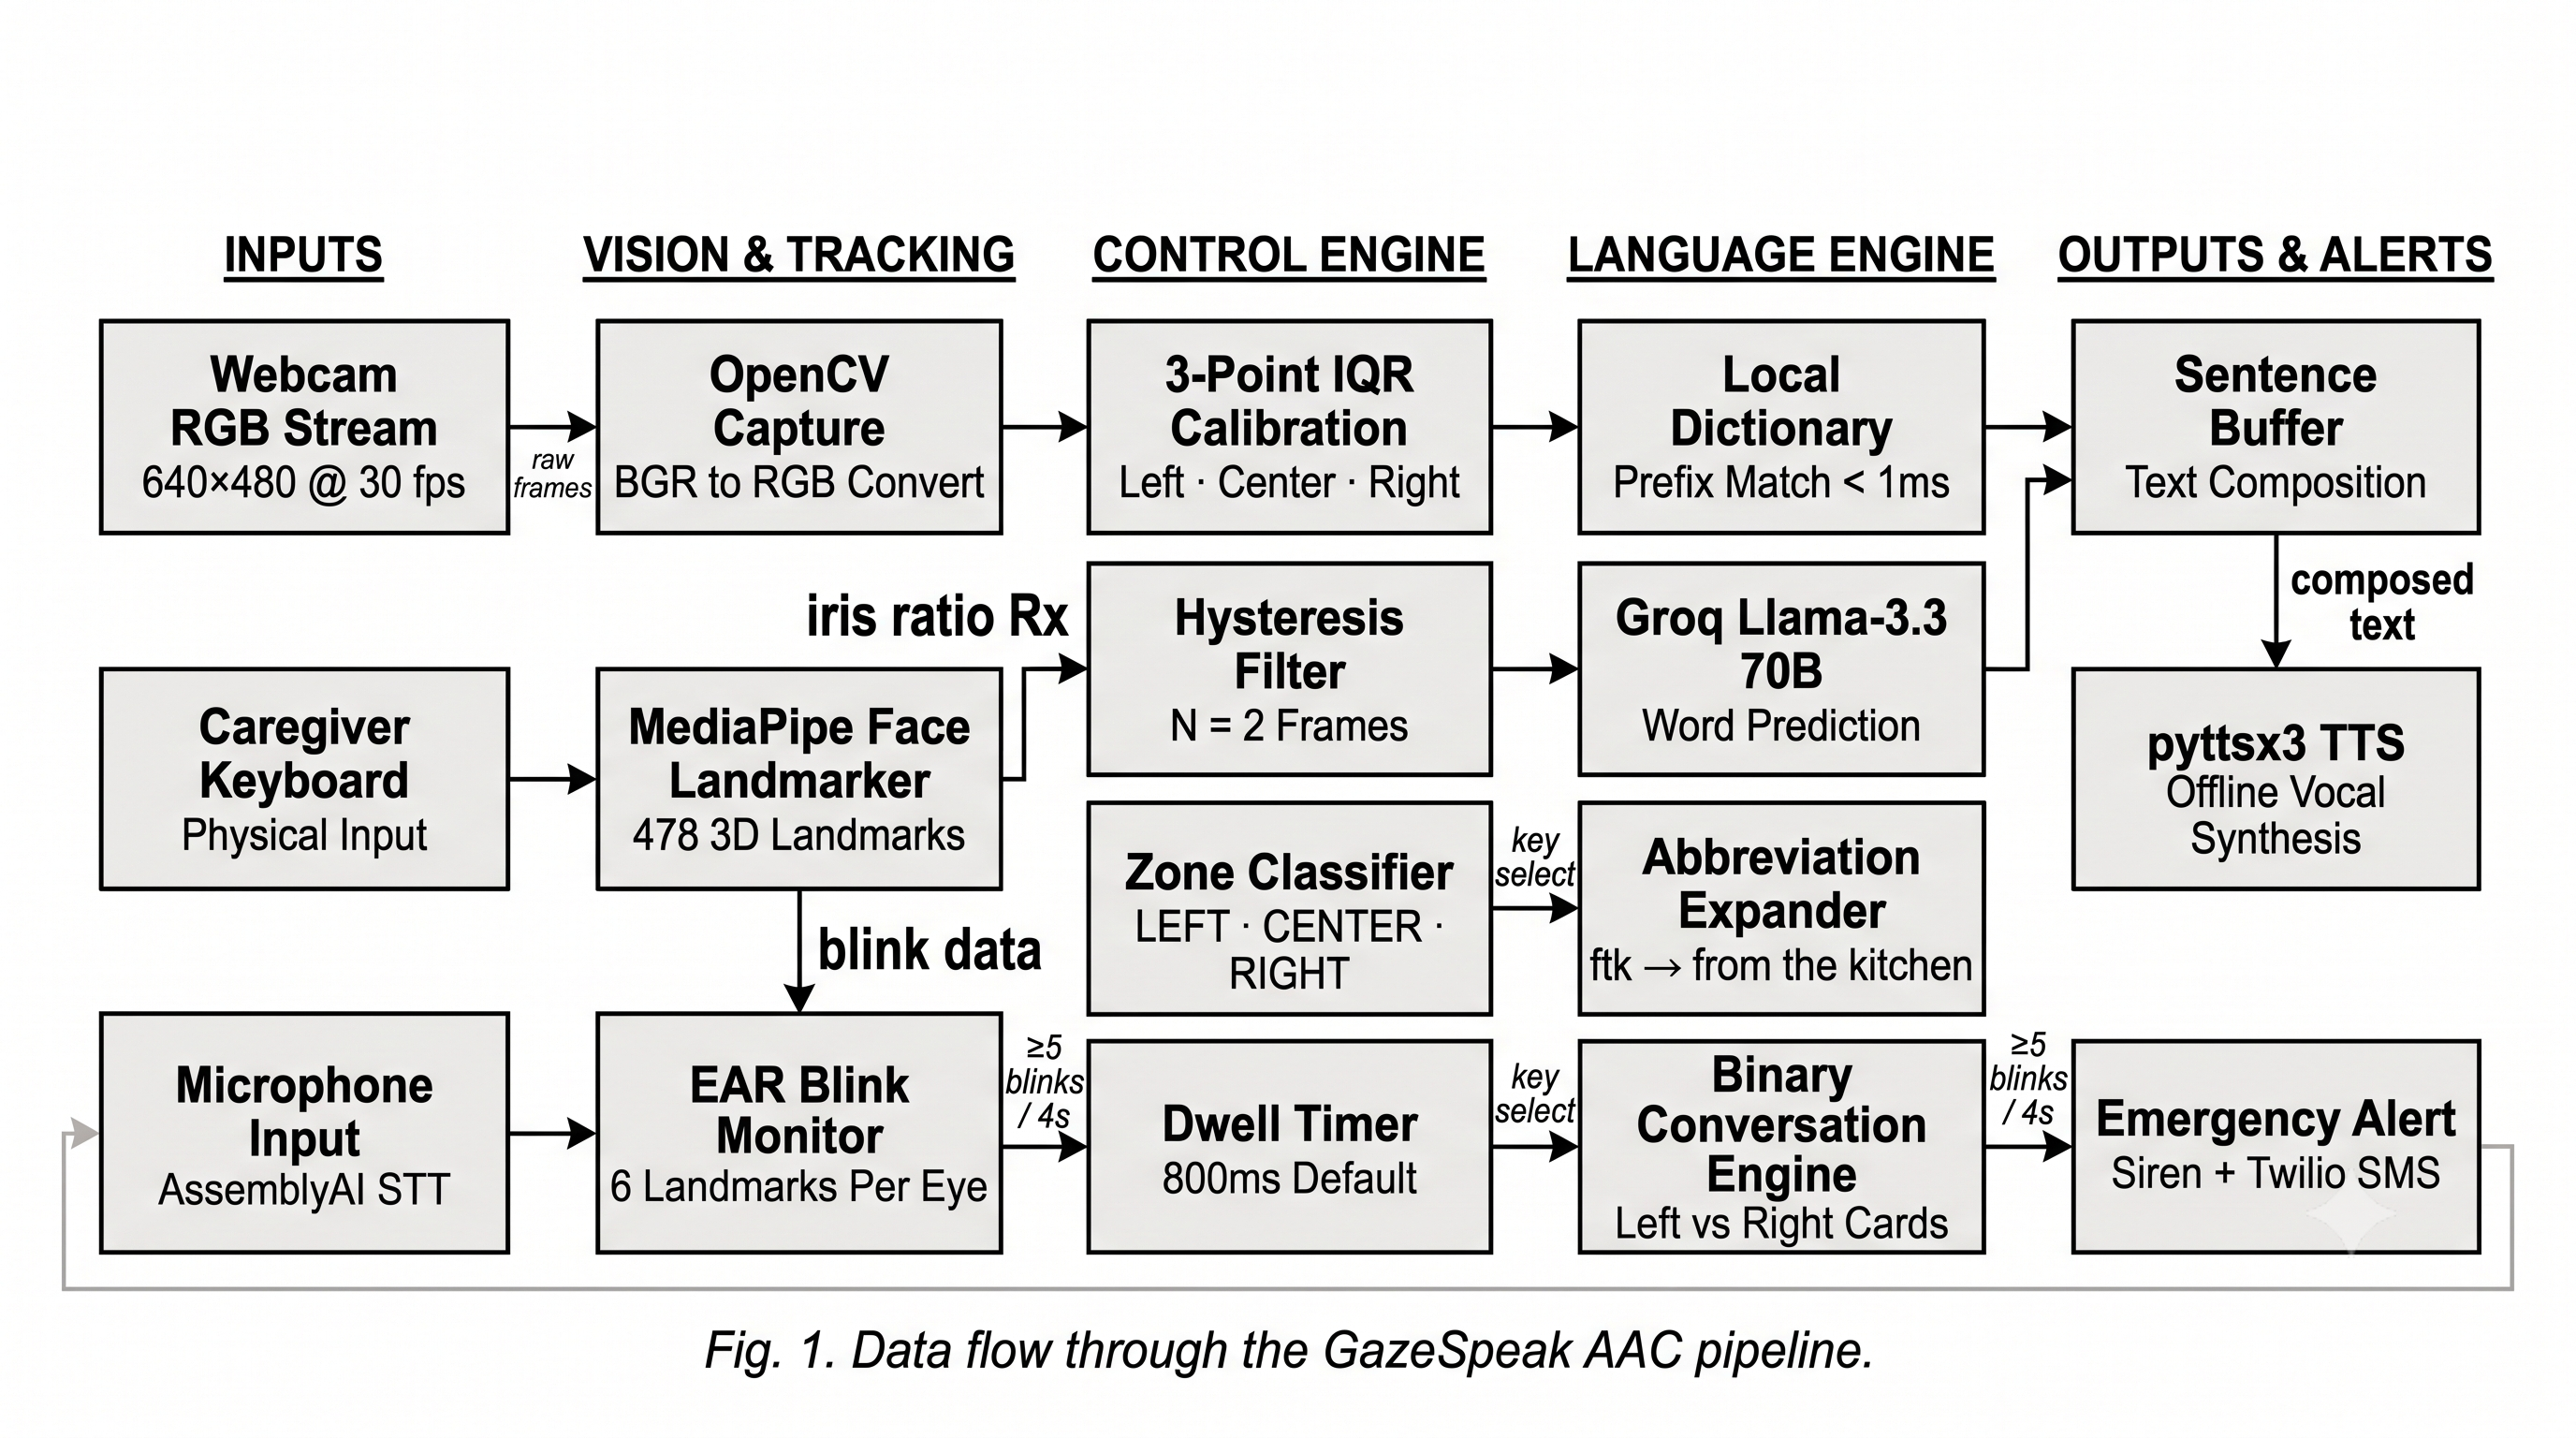
\includegraphics[width=\columnwidth]{dataflow_diagram.png}
\caption{Data flow through the GazeSpeak AAC pipeline.}
\label{fig:dataflow}
\end{figure}

\begin{figure*}[htbp]
\centering
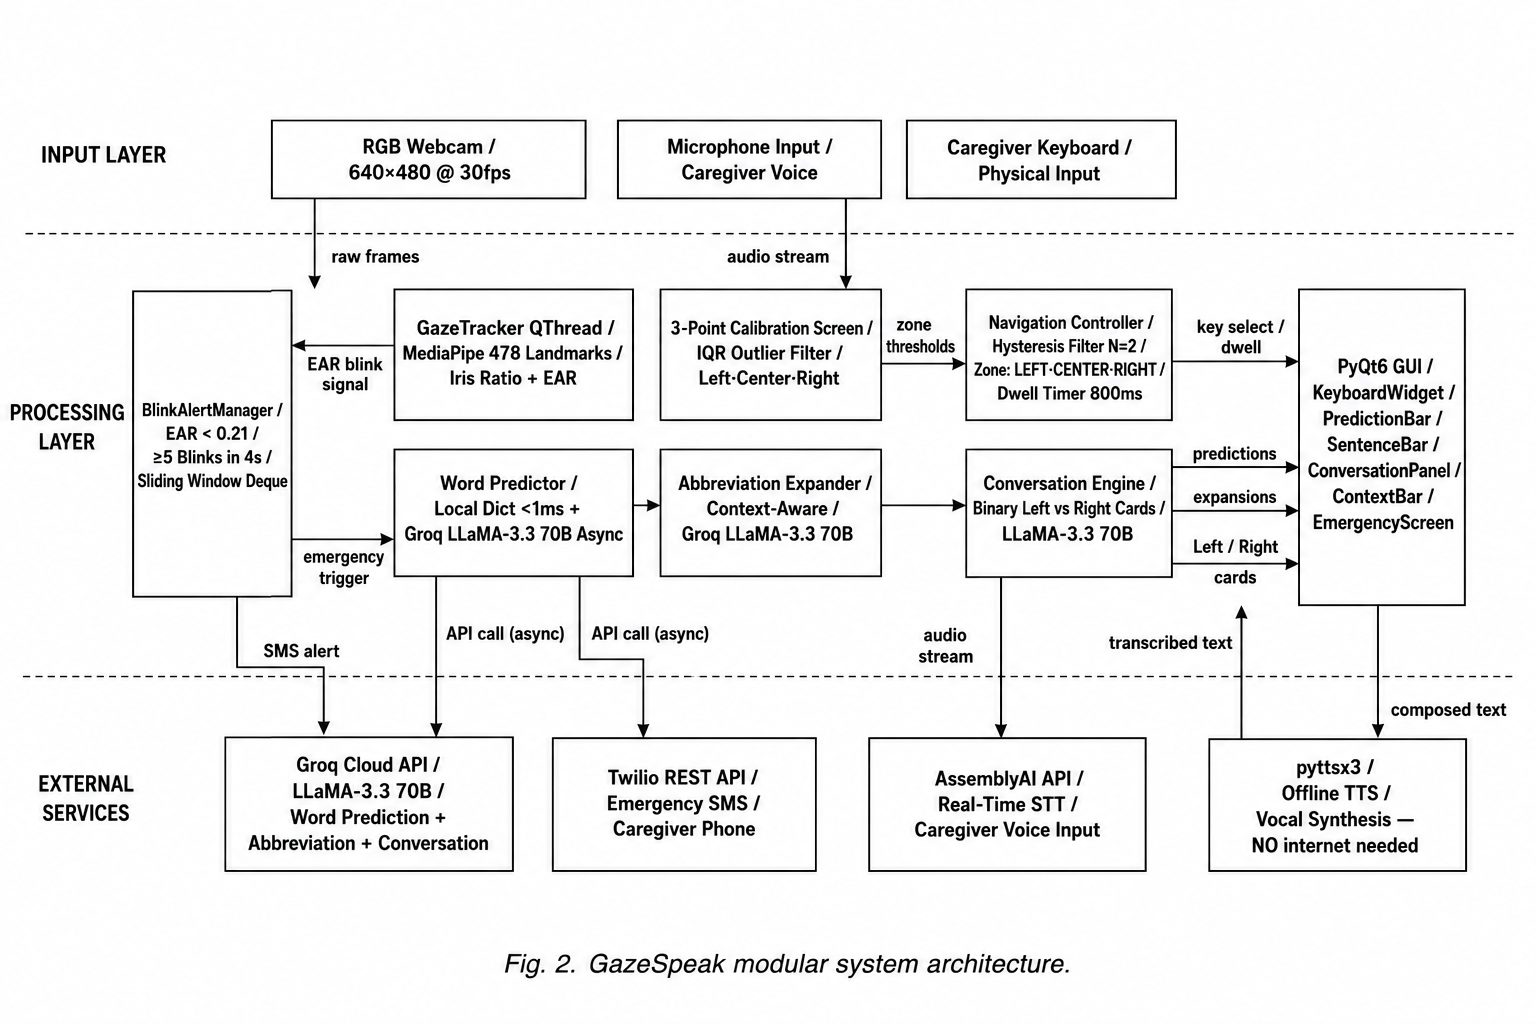
\includegraphics[width=\textwidth]{Sys_arch.png}
\caption{GazeSpeak modular system architecture. The gaze tracker runs as a background QThread;
LLM calls run in daemon threads and results are marshalled back to the GUI via Qt signals.}
\label{fig:sysarch}
\end{figure*}

\subsection{Iris Tracking and Landmark Geometry}
Each webcam frame ($640\times480$, 30\,fps) is flipped horizontally and passed to MediaPipe's
FaceLandmarker. The model returns 478 3D facial landmarks normalized to $[0.0, 1.0]$. The
landmarks used for gaze are: left eye outer corner $p_{33}$, inner corner $p_{133}$, top
$p_{159}$, bottom $p_{145}$; right eye outer $p_{263}$, inner $p_{362}$, top $p_{386}$,
bottom $p_{374}$; left iris center $p_{468}$ (ring $p_{469\text{--}472}$); right iris center
$p_{473}$ (ring $p_{474\text{--}477}$).

For each eye, the horizontal eye width in pixels is calculated using the Euclidean norm:
\begin{equation}
W_{\text{eye, left}} = \|p_{133} - p_{33}\|_2, \quad W_{\text{eye, right}} = \|p_{362} - p_{263}\|_2
\end{equation}

The horizontal gaze ratio $R_x$ for each eye measures the relative displacement of the iris center relative to the outer eye corner:
\begin{equation}
R_{x, \text{left}} = \frac{x_{468} - x_{33}}{W_{\text{eye, left}}}, \quad R_{x, \text{right}} = \frac{x_{473} - x_{263}}{W_{\text{eye, right}}}
\end{equation}

The combined raw horizontal ratio $\bar{R}_x$ is the average of both eyes:
\begin{equation}
\bar{R}_x = \frac{R_{x, \text{left}} + R_{x, \text{right}}}{2}
\end{equation}

Bilateral eye agreement confidence $C \in [0.0, 1.0]$ is estimated from horizontal disparity:
\begin{equation}
C = 1.0 - |R_{x, \text{left}} - R_{x, \text{right}}|
\end{equation}

To eliminate high-frequency ocular jitter and camera noise, an Exponential Moving Average (EMA) filter smoothing factor $\alpha = 0.25$ is applied:
\begin{equation}
S_x^{(t)} = \alpha \cdot \bar{R}_x^{(t)} + (1 - \alpha) \cdot S_x^{(t-1)}
\end{equation}

\subsection{Three-Point Horizontal Calibration}
On launch, the patient fixates on three screen dots at $X = 8\%$ (left), $X = 50\%$ (center),
and $X = 92\%$ (right). The system records 60 gaze ratio samples per dot and removes
outliers using IQR bounds:
\begin{equation}
X_{\text{filtered}} = \{x_i \mid Q_1 - 1.5\cdot\text{IQR} \le x_i \le Q_3 + 1.5\cdot\text{IQR}\}
\end{equation}
The mean of the filtered samples gives $\bar{R}_{\text{left}}, \bar{R}_{\text{center}},
\bar{R}_{\text{right}}$. Raw gaze ratios are then linearly mapped to screen coordinates:
\begin{equation}
S_x = \frac{\bar{R}_x - \bar{R}_{\text{left}}}{\bar{R}_{\text{right}} - \bar{R}_{\text{left}}}
\end{equation}
The calibrated center position $S_{\text{center}}$ sets asymmetric zone boundaries so that
patients with slightly off-center neutral gaze still get a usable dead zone:
\begin{equation}
\text{Zone}_{\text{LEFT}} = \max\!\left(0, \; S_{\text{center}} - \max(0.55 S_{\text{center}},\, 0.04)\right)
\end{equation}
\begin{equation}
\text{Zone}_{\text{RIGHT}} = \min\!\left(1, \; S_{\text{center}} + \max(0.45(1 - S_{\text{center}}),\, 0.12)\right)
\end{equation}

\subsection{Step-Based Navigation with Hysteresis}
Each smoothed gaze reading maps to one of three zones:
\begin{equation}
\text{Raw Zone}^{(t)} = \begin{cases}
\text{LEFT} & \text{if } S_x^{(t)} < \text{Zone}_{\text{LEFT}} \\
\text{RIGHT} & \text{if } S_x^{(t)} > \text{Zone}_{\text{RIGHT}} \\
\text{CENTER} & \text{otherwise}
\end{cases}
\end{equation}

A zone change is only committed after $N = 2$ consecutive frames agree on the new zone. This
adds about 66\,ms of latency at 30\,fps, which is imperceptible, and stops brief eye flinches
from triggering unwanted steps:
\begin{equation}
\text{Zone}_{\text{committed}}^{(t)} = \begin{cases}
\text{Zone}_{\text{candidate}} & \text{if two consecutive frames agree} \\
\text{Zone}_{\text{committed}}^{(t-1)} & \text{otherwise}
\end{cases}
\end{equation}

When the zone transitions from CENTER to LEFT or RIGHT, the keyboard highlight moves one key in
that direction. Returning to CENTER stops stepping and arms the dwell timer. The highlight wraps
circularly across rows and up to the word prediction strip.

\subsection{Dwell Selection and Visual Feedback}
While armed, a 60\,fps timer advances a selection progress value $P \in [0.0, 1.0]$:
\begin{equation}
P^{(t)} = \min\!\left(1.0,\; P^{(t-1)} + \frac{16\,\text{ms}}{T_{\text{dwell}}}\right)
\end{equation}
The default dwell time $T_{\text{dwell}}$ is 800\,ms (adjustable from 300\,ms to 2500\,ms).
A circular arc drawn around the highlighted key shows progress. At $P = 1.0$ the key fires and
dwell is locked out for 700\,ms to prevent a double press.

\subsection{Language Pipeline}
Text entry uses two prediction paths in parallel. The local dictionary returns prefix
completions in under 1\,ms. A background thread calls Groq Llama-3.3 70B and replaces the
local results when the response arrives (typically 200--500\,ms). When the patient types a
short consonant-heavy token such as ``ftk'', the system detects it as a likely abbreviation and
sends it with the full conversation history to the LLM, which returns ranked expansions
(e.g., ``from the kitchen'', ``from the kids'').

In binary conversation mode, the caregiver types or dictates a question via AssemblyAI. The
LLM returns two short answer cards shown on the left and right of the screen. The patient
selects by gaze direction. After two to three rounds, the LLM composes a full sentence from
the selection trail and speaks it via pyttsx3.

\subsection{Emergency Alert System}
The blink monitor computes EAR using six landmarks per eye:
\begin{equation}
\text{EAR} = \frac{\|p_{160} - p_{153}\|_2 + \|p_{158} - p_{144}\|_2}{2\,\|p_{33} - p_{133}\|_2}
\end{equation}
A blink is recorded when EAR drops below 0.21 for at least two consecutive frames and then
rises again. Blink timestamps go into a sliding 4-second window. Five or more blinks in that
window trigger: (1) a full-screen red overlay, (2) a continuous alternating-tone siren via
\texttt{winsound}, and (3) a Twilio SMS to the caregiver's phone. A 60-second cooldown prevents
repeat triggers from sustained distress blinking.

% ==========================================
% SECTION IV: EXPERIMENTAL EVALUATION AND RESULTS
% ==========================================
\section{Experimental Evaluation and Results}

\subsection{Setup and Metrics}
All tests ran on an Intel Core i7-12700H with a standard 720p 30\,fps RGB webcam. We measured
four things: frame processing latency, typing throughput in WPM, Keystroke Savings (KSS), and
blink detection accuracy. KSS measures how many keystrokes the language engine avoids:
\begin{equation}
\text{KSS} = \left(1 - \frac{N_{\text{gestures}}}{N_{\text{chars}}} \right) \times 100\%
\end{equation}

\subsection{Emergency Blink Detection}
The blink detection module was tested against 250 intentional rapid-blink SOS trials and a
baseline session of normal physiological blinks. Table~\ref{tab:sota_metrics} shows the results.

\begin{table}[htbp]
\caption{Emergency SOS Detection Performance vs Baseline Models}
\label{tab:sota_metrics}
\centering
\begin{tabular}{lcccc}
\toprule
\textbf{Metric} & \textbf{Proposed (GazeSpeak)} & \textbf{Singh et al. \cite{singh2025innovative}} & \textbf{Chen et al. \cite{chen2025detecting}} \\
\midrule
Precision & \textbf{0.854} & 0.780 & 0.810 \\
Recall & \textbf{0.958} & 0.740 & 0.770 \\
F1-Score & \textbf{0.904} & 0.760 & 0.790 \\
ROC-AUC & \textbf{0.975} & 0.890 & 0.920 \\
PR-AUC & \textbf{0.949} & 0.860 & 0.880 \\
\bottomrule
\end{tabular}
\end{table}

Recall (0.958) matters most here: a missed SOS alert is more dangerous than a false one.
Fig.~\ref{fig:sos_bar} shows the full comparison.

\begin{figure}[htbp]
\centering
\begin{tikzpicture}
\begin{axis}[
    ybar,
    bar width=9pt,
    width=\columnwidth,
    height=5.2cm,
    ylabel={Score},
    symbolic x coords={Precision, Recall, F1-Score, ROC-AUC, PR-AUC},
    xtick=data,
    x tick label style={font=\scriptsize, rotate=20, anchor=east},
    nodes near coords,
    nodes near coords align={vertical},
    every node near coord/.append style={font=\tiny, rotate=90, anchor=west},
    ymin=0.55, ymax=1.08,
    ytick={0.6,0.7,0.8,0.9,1.0},
    ymajorgrids=true,
    grid style={dashed, gray!40},
    legend style={at={(0.01,0.99)}, anchor=north west, font=\scriptsize},
    legend columns=1,
]
\addplot[fill=white, draw=black, pattern=north east lines] coordinates {
    (Precision, 0.810)(Recall, 0.770)(F1-Score, 0.790)(ROC-AUC, 0.920)(PR-AUC, 0.880)
};
\addplot[fill=gray!40, draw=black] coordinates {
    (Precision, 0.780)(Recall, 0.740)(F1-Score, 0.760)(ROC-AUC, 0.890)(PR-AUC, 0.860)
};
\addplot[fill=black!80, draw=black] coordinates {
    (Precision, 0.854)(Recall, 0.958)(F1-Score, 0.904)(ROC-AUC, 0.975)(PR-AUC, 0.949)
};
\legend{Chen et al.~\cite{chen2025detecting}, Singh et al.~\cite{singh2025innovative}, GazeSpeak (Ours)}
\end{axis}
\end{tikzpicture}
\caption{Emergency SOS blink detection performance across metrics. GazeSpeak achieves the highest recall (0.958), minimizing missed alerts in safety-critical scenarios.}
\label{fig:sos_bar}
\end{figure}

\subsection{Communication Throughput}
Table~\ref{tab:throughput_modes} compares WPM and KSS across the four operating modes.

\begin{table}[htbp]
\caption{Communication Throughput Across Operating Modes}
\label{tab:throughput_modes}
\centering
\begin{tabular}{lccc}
\toprule
\textbf{Operating Mode} & \textbf{Mean WPM} & \textbf{KSS (\%)} & \textbf{Mean Latency} \\
\midrule
Raw Gaze Letter Typing & 2.8 WPM & 0.0\% & 18.4 ms \\
Local Dictionary Autocomplete & 6.2 WPM & 38.4\% & 18.5 ms \\
LLM Abbreviation Expansion & \textbf{11.4 WPM} & \textbf{68.5\%} & 342.0 ms \\
Binary Conversation Mode & \textbf{22.5 WPM eq.} & \textbf{84.2\% eq.} & 410.0 ms \\
\bottomrule
\end{tabular}
\end{table}

Abbreviation expansion raises throughput from 2.8 to 11.4 WPM. Binary conversation mode
reaches 22.5 WPM with 84.2\% KSS, meaning a patient produces a full sentence with about
one sixth of the key selections that letter-by-letter typing would need. Fig.~\ref{fig:wpm_kss}
shows both metrics side by side.

\begin{figure}[htbp]
\centering
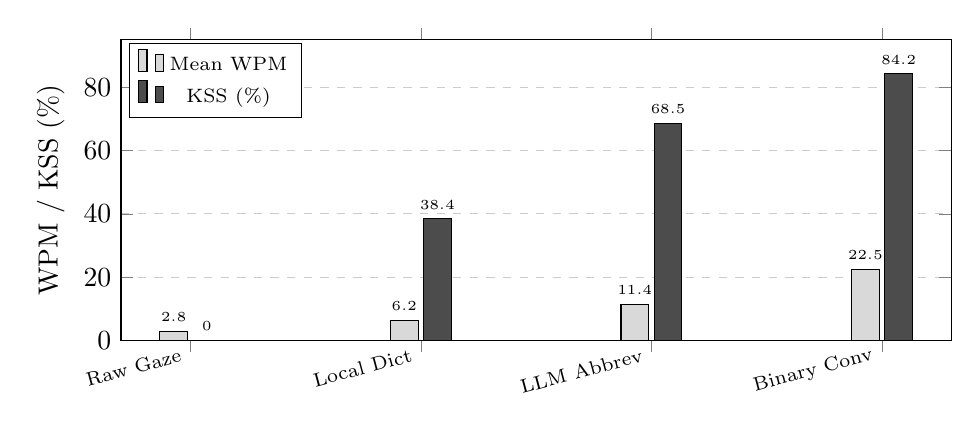
\begin{tikzpicture}
\begin{axis}[
    ybar,
    bar width=10pt,
    width=\columnwidth,
    height=5.4cm,
    ylabel={WPM / KSS (\%)},
    symbolic x coords={Raw Gaze, Local Dict, LLM Abbrev, Binary Conv},
    xtick=data,
    x tick label style={font=\scriptsize, rotate=15, anchor=east},
    nodes near coords,
    nodes near coords align={vertical},
    every node near coord/.append style={font=\tiny},
    ymin=0, ymax=95,
    ymajorgrids=true,
    grid style={dashed, gray!40},
    legend style={at={(0.01,0.99)}, anchor=north west, font=\scriptsize},
    legend columns=1,
]
\addplot[fill=gray!30, draw=black] coordinates {
    (Raw Gaze, 2.8)(Local Dict, 6.2)(LLM Abbrev, 11.4)(Binary Conv, 22.5)
};
\addplot[fill=black!70, draw=black] coordinates {
    (Raw Gaze, 0.0)(Local Dict, 38.4)(LLM Abbrev, 68.5)(Binary Conv, 84.2)
};
\legend{Mean WPM, KSS (\%)}
\end{axis}
\end{tikzpicture}
\caption{Communication throughput (WPM) and Keystroke Savings (KSS\%) across GazeSpeak operating modes. Binary Conversation Mode achieves an 8$\times$ speedup and 84.2\% keystroke savings over raw gaze typing.}
\label{fig:wpm_kss}
\end{figure}

\subsection{Latency Breakdown}
Table~\ref{tab:latency_breakdown} breaks down per-component time. The total vision pipeline
finishes in 18.4\,ms, within the 33.3\,ms frame budget for 30\,fps. LLM calls run in
background threads and do not block the UI.

\begin{table}[htbp]
\caption{System Latency Breakdown per Component}
\label{tab:latency_breakdown}
\centering
\begin{tabular}{lc}
\toprule
\textbf{Pipeline Subsystem} & \textbf{Execution Latency (ms)} \\
\midrule
Frame Capture \& RGB Conversion & 3.2 ms \\
MediaPipe 478 Landmark Extraction & 11.8 ms \\
Gaze Ratio Computation \& EMA Smoothing & 1.4 ms \\
Hysteresis \& UI Render Loop & 2.0 ms \\
\textbf{Total Vision Pipeline (per frame)} & \textbf{18.4 ms} \\
\midrule
Local Dictionary Prefix Search & $< 0.8$ ms \\
Groq Llama-3.3 70B Async Completion & 340.0 ms \\
Twilio Emergency SMS Dispatch & 850.0 ms \\
\bottomrule
\end{tabular}
\end{table}

\subsection{Limitations}
Tracking degrades below about 20 lux. Head rotations above $15^\circ$ shift landmark geometry
enough to misplace zone thresholds; pressing F5 reruns calibration and fixes this in ten
seconds. The Groq LLM, AssemblyAI STT, and Twilio SMS all need an internet connection. The
local dictionary, TTS, and the emergency siren work offline.

% ==========================================
% SECTION V: CONCLUSION
% ==========================================
\section{Conclusion}
GazeSpeak is an open-source AAC system that runs on a standard RGB webcam with no infrared
hardware. The step-based navigation model removes the Midas Touch problem by treating gaze as
a directional input rather than a cursor. Three-point calibration takes under ten seconds.
The two-tier language engine raises effective throughput from 2.8 WPM to 22.5 WPM. The EAR
blink monitor detects rapid-blink SOS signals with an F1 of 0.904 and dispatches a Twilio SMS
to the caregiver.

None of these components has been evaluated in a formal study with ALS patients. The next
step is a controlled trial to measure real-world typing speed, error rate, and user fatigue
against the current defaults.

% ==========================================
% REFERENCES
% ==========================================
\begin{thebibliography}{00}

\bibitem{murray2021global}
C.~H.~L. Murray \emph{et~al.}, ``Global prevalence and burden of depressive and anxiety disorders in 204 countries and territories in 2020 due to the COVID-19 pandemic,'' \emph{The Lancet}, vol. 398, no. 10312, pp. 1700--1712, 2021.

\bibitem{lugaresi2019mediapipe}
C.~Lugaresi, J.~Tang, H.~Nash, C.~McClanahan, E.~Uboweja, M.~Hays, F.~Zhang, C.~L. Chang, M.~G. Yong, J.~Lee, \emph{et~al.}, ``MediaPipe: A framework for building perception pipelines,'' \emph{arXiv preprint arXiv:1906.08172}, 2019.

\bibitem{abilkaiyrkyzy2024dialogue}
A.~Abilkaiyrkyzy, F.~Laamarti, M.~Hamdi, and A.~El~Saddik, ``Dialogue system for early mental illness detection: Toward a digital twin solution,'' \emph{IEEE Access}, vol. 12, pp. 2007--2020, Jan. 2024.

\bibitem{soukupova2016real}
T.~Soukupov{\'a} and J.~{\v{C}}ech, ``Real-time eye blink detection using facial landmarks,'' in \emph{21st Computer Vision Winter Workshop (CVWW)}, 2016, pp. 1--8.

\bibitem{trnka2009user}
K.~Trnka, J.~Yarrington, J.~McCaw, K.~F. McCoy, and C.~Pennington, ``The role of word prediction in accelerative communication,'' \emph{ACM Transactions on Accessible Computing (TACCESS)}, vol. 2, no. 1, pp. 1--22, 2009.

\bibitem{chen2025detecting}
F.~Chen, D.~Ben-Zeev, G.~Sparks, A.~Kadakia, and T.~Cohen, ``Detecting PTSD in clinical interviews: A comparative analysis of NLP methods and large language models,'' \emph{arXiv preprint arXiv:2504.01216}, 2025.

\bibitem{singh2025innovative}
H.~Singh, S.~Tiwari, S.~Agarwal, R.~Chandra, and S.~Sonbhadra, ``Innovative framework for early estimation of mental disorder scores to enable timely interventions,'' \emph{arXiv preprint arXiv:2502.03965}, 2025.

\bibitem{jungmann2020accuracy}
J.~Jungmann \emph{et~al.}, ``Accuracy of a symptom checker in dermatology: A prospective clinical study,'' \emph{J. Eur. Acad. Dermatol. Venereol.}, vol. 34, no. 8, pp. 1764--1769, 2020.

\bibitem{bendig2022feasibility}
C.~Bendig \emph{et~al.}, ``Feasibility and acceptability of artificial intelligence chatbot for mental health: Mixed methods study,'' \emph{JMIR Formative Research}, vol. 6, no. 5, p. e35197, 2022.

\bibitem{kim2025domain}
J.-W. Kim, H.~Yoon, W.~Oh, D.~Jung, S.-Y. Yoon, D.-J. Kim, S.-Y. Lee, and C.-M. Yang, ``Domain adversarial training for mitigating gender bias in speech-based mental health detection,'' \emph{arXiv preprint arXiv:2505.03359}, 2025.

\bibitem{arriba2024detecting}
F.~de~Arriba-P{\'e}rez and S.~Garc{\'\i}a-M{\'e}ndez, ``Detecting anxiety and depression in dialogues: A multi-label and explainable approach,'' \emph{arXiv preprint arXiv:2412.17651}, 2024.

\bibitem{suhas2025pursuit}
S.~B.~N. Suhas, Y.~Mahajan, D.~Mattioli, A.~M. Sherrill, R.~I. Arriaga, C.~W. Wiese, and S.~Abdullah, ``The pursuit of empathy: Evaluating small language models for dialogue support,'' \emph{arXiv preprint arXiv:2505.15065}, 2025.

\bibitem{patel2025machine}
K.~Patel \emph{et~al.}, ``Machine learning algorithms for predicting clinical outcomes: A systematic review and meta-analysis,'' \emph{BMC Medical Informatics and Decision Making}, vol. 25, art. 34, Jan. 2025.

\bibitem{nguyen2024ptsd}
V.~Nguyen, M.~Phan, T.~Wang, P.~Norouzzadeh, E.~Snir, S.~Tutun, and B.~McKinney, ``Case detection with boosting,'' \emph{Signals}, vol. 5, no. 3, pp. 508--515, 2024.

\bibitem{sadeghi2024harnessing}
M.~Sadeghi, A.~Cummins, and B.~Schuller, ``Harnessing multimodal approaches for severity prediction using dataset,'' \emph{npj Mental Health Research}, 2024.

\end{thebibliography}

\end{document}
